\documentclass[runningheads]{llncs}
\usepackage[T1]{fontenc}
\usepackage{graphicx}
\usepackage{booktabs}
\usepackage{url}
\usepackage{bbding}
\usepackage{xcolor}
\usepackage[normalem]{ulem}

% ---- Revision tracking against the reviewed submission (2026-06-14) ----
% \rev{...}  = added or changed text (red)
% \del{...}  = deleted text (red strikeout)
% \dnote{...} = editorial note (red, brackets)
% Wrap ALL future edits in these macros so co-authors can track changes.
% Set \showdifffalse to produce the clean camera-ready (marks vanish).
\newif\ifshowdiff
\showdifftrue
\ifshowdiff
  % Japanese support for the reviewer-facing notes (tracking build only;
  % the clean camera-ready build never loads these packages).
  \usepackage{xeCJK}
  \setCJKmainfont{Hiragino Kaku Gothic ProN}
  \newcommand{\rev}[1]{\textcolor{red}{#1}}
  \newcommand{\del}[1]{\textcolor{red}{\sout{#1}}}
  \newcommand{\dnote}[1]{\textcolor{red}{[\textit{#1}]}}
  \newcommand{\revfloat}{\color{red}}
  \newcommand{\cmpredheader}{& \multicolumn{6}{c}{\del{\textbf{Predicted}}} \\ \cmidrule(lr){2-7}}
  \newcommand{\zsperclassrows}{\del{DEPRESSIVE F1} & \del{\textbf{0.738}} & \del{0.734} & \del{$-$0.004} \\ \del{STABLE F1} & \del{0.600} & \del{\textbf{0.716}} & \del{$+$0.116} \\ \del{HYPOMANIC F1} & \del{0.500} & \del{0.500} & \del{$\pm$ 0.000} \\ \del{MANIC F1} & \del{0.000} & \del{\textbf{0.125}} & \del{$+$0.125} \\}
\else
  \newcommand{\rev}[1]{#1}
  \newcommand{\del}[1]{}
  \newcommand{\dnote}[1]{}
  \newcommand{\revfloat}{}
  \newcommand{\cmpredheader}{}
  \newcommand{\zsperclassrows}{}
\fi

% Long unbreakable \texttt identifiers (e.g. TOWARDS_DEPRESSION) otherwise
% produce overfull lines; allow modest extra inter-word stretch instead.
\setlength{\emergencystretch}{3em}

\begin{document}

\title{Few-Shot Prompt-Based Longitudinal Mood-State Analysis of Bipolar Disorder on Social Media}
\titlerunning{Few-Shot BD Mood-State Analysis}

\author{Jiefeng Lin\textsuperscript{(\Envelope)}\orcidID{0000-0003-1800-0052} \and
Koichiro Watanabe\orcidID{0000-0002-3543-2159} \and
Shuntaro Yada\orcidID{0000-0002-6209-1054}}
\authorrunning{J. Lin et al.}

\institute{University of Tsukuba, 1-2 Kasuga, Tsukuba, Ibaraki 305-8550, Japan\\
\email{\{lin.jiefeng.tkb\_ge,watanabe.koichiro.ge\}@u.tsukuba.ac.jp}\\
\email{yada@slis.tsukuba.ac.jp}}

\maketitle

\ifshowdiff
\begin{center}
\fbox{\parbox{0.92\textwidth}{\color{red}\footnotesize
\textbf{改稿トラッキング版（提出版ではありません）。}赤字は査読時の投稿版（6月14日）から追加・変更した箇所、\sout{赤の取り消し線}は削除した箇所を示します。本文は投稿版の文言を基準とし、変更は査読コメントへの対応・数値の修正・出版要件によるものに限っています。マークしていないもの：著者・所属・倫理承認番号の復元（査読用の匿名化の解除）、テンプレート移行に伴う純粋に組版上の差異。なお、Gemini の引用は 2024 年の Gemini ファミリー報告から Gemini~3.1~Pro の Model Card（2026 年）に差し替えました。参考文献リストは BibTeX の自動生成のためマーク不可ですが、ModernBERT 論文（Warner et al.）に DOI とページ番号を補記しました。}}
\end{center}
\fi

\begin{abstract}
Bipolar disorder (BD) is frequently misdiagnosed as major depressive disorder, and monitoring mood-state \emph{transitions} over time is critical for timely intervention. Although existing social media datasets for BD research provide binary diagnostic labels or per-post mood scores, few capture how mood states evolve over time. Because expert annotation is costly and fine-tuning requires scarce labeled data, we propose a few-shot prompt-based LLM method that requires no task-specific training \rev{data at inference time}. The annotation schema is grounded in DSM-5 episode criteria and accompanied by eight synthetic few-shot examples, making the method directly applicable to other BD corpora. The method labels posts at two granularities: per-post mood state and 14-day period-level trends (dominant state, trend direction, change points), enabling trajectory modeling that per-post labels alone cannot support. Post-level classification is externally validated against the BD-Risk dataset~\cite{lee2024detecting} on a held-out, author-disjoint, stratified subset of 145 posts, achieving macro F1 of 0.519 with high depressive recall (87.9\%) and lower manic-pole recall (35.7\% hypomanic, 6.7\% manic). Six error patterns are characterized, \del{including} \rev{alongside} a structural label-text consistency issue at the manic pole that bounds achievable manic recall. \rev{A cross-model evaluation confirms schema portability across four additional LLMs.} Using Gemini 3.1 Pro, we apply the method to 105 self-identified BD users on BD-focused subreddits (1,794 14-day periods, 15,423 posts and comments, April 2019--May 2026), observing depressive-pole predominance broadly consistent with clinical expectations for BD-related online discussion.

\keywords{Bipolar Disorder \and Large Language Models \and Few-Shot Prompting \and Social Media \and Clinical NLP \and Mood Trajectory.}
\end{abstract}

\section{Introduction}

Bipolar disorder (BD) is characterized by recurrent episodes of mania, hypomania, and depression, affecting 1--2\% of the global population~\cite{grande2016bipolar}. An estimated 17--50\% of BD cases are initially misdiagnosed as major depressive disorder (MDD), because patients typically seek help during depressive episodes and may not recognize manic or hypomanic states as pathological~\cite{hirschfeld2002guideline,vieta2018misdiagnosis}. This misdiagnosis leads to inappropriate treatment (e.g., antidepressant monotherapy, which may trigger manic switching) and delays proper intervention.

Social media platforms such as Reddit host BD communities (e.g., r/bipolar, r/BipolarReddit) where users openly discuss symptoms, treatment, and daily functioning. Prior work has used these data for BD and MDD classification~\cite{cohan2018smhd,coppersmith2015clpsych,sekulic2018not}, yet existing datasets provide only per-user binary diagnosis labels (BD vs.~MDD) or aggregate user-level risk scores, neither of which records how individual mood states evolve across posts. Few resources offer post-level mood state labels tracked longitudinally, limiting computational research on mood trajectories and, in turn, on BD progression and early intervention.

Constructing expert-annotated BD corpora is costly: mood-state labeling requires psychiatric expertise, and the scarcity of labeled data makes fine-tuning approaches difficult to scale. At the same time, recent advances in large language models (LLMs) suggest that they can follow human-written guidelines with reasonable accuracy on text annotation tasks~\cite{gilardi2023chatgpt}. This motivates our approach: if LLMs can internalize clinical guidelines presented in a prompt, then a carefully designed DSM-5-grounded prompt with synthetic few-shot examples should enable mood-state annotation \emph{without task-specific fine-tuning or labeled training data \rev{at inference time}}, making the method directly applicable to new BD corpora.

Recent work has applied LLMs to mental health NLP tasks~\cite{xu2024mental,yang2024mentallama}; however, whether they can classify BD mood states at expert-level accuracy, especially manic-pole states that are difficult to detect from text, has not been established.

This paper proposes a few-shot prompt-based LLM method for longitudinal mood-state analysis of BD on social media and demonstrates its application to a Reddit cohort. We collect Reddit posts from BD-focused subreddits\del{ (r/bipolar, r/BipolarReddit, r/bipolar2)}, targeting users who self-identify as having a BD diagnosis, and annotate them at two granularities: (1) per-post mood state\del{ (\emph{Depressive}, \emph{Stable}, \emph{Hypomanic}, \emph{Manic})} and (2) 14-day period-level mood trends\del{ (dominant state, trend direction, change points)}. \del{The annotation schema follows DSM-5 episode criteria and is implemented as an LLM pipeline (Gemini 3.1 Pro).} We validate the post-level annotations against the BD-Risk dataset~\cite{lee2024detecting} on a held-out, author-disjoint, stratified subset of 145 posts\del{, achieving macro F1 of 0.519 with 87.9\% depressive recall, 35.7\% hypomanic recall, and 6.7\% manic recall}\rev{, observing substantially higher depressive-pole than manic-pole recall}. The recall asymmetry across poles reflects both a known model property (manic-side states often manifest through described behaviors rather than affective tone) and a structural label-text consistency issue with the source dataset's manic-pole labels.

Our contributions:
\begin{enumerate}
\item \textbf{Method:} A DSM-5-grounded few-shot prompt schema for LLM-based mood-state annotation at two temporal granularities (per-post state and 14-day period-level trend), requiring no fine-tuning or labeled training data \rev{at inference time}.
\item \textbf{Evaluation:} External validation of post-level state classification against the BD-Risk \del{expert-labeled} \rev{expert-validated} dataset~\cite{lee2024detecting} on a held-out, author-disjoint, stratified subset, with macro F1 of 0.519 (87.9\% depressive recall, 35.7\% hypomanic recall, 6.7\% manic recall), complemented by a zero-shot baseline comparison\del{ and a cross-model feasibility probe}\rev{, a supervised fine-tuning baseline, and a cross-model portability evaluation across five additional LLMs from five providers (macro F1 0.432--0.564 for the four completing models)}.
\item \textbf{Demonstration:} Application of the method to 105 self-identified BD users from BD-focused subreddits (1,794 14-day periods, 15,423 posts and comments spanning April 2019 through May 2026), producing longitudinal mood trajectory annotations with distributions broadly consistent with clinical expectations for BD-related online discussion.
\end{enumerate}

\section{Related Work}

\subsection{Longitudinal Mood Monitoring in BD}

Clinical efforts to track BD mood trajectories rely heavily on ecological momentary assessment (EMA) and digital phenotyping with smartphone sensors and self-report apps~\del{\cite{faurholt2018smartphone,torous2016new}}\rev{\cite{faurholt2018smartphone}}. \del{These approaches yield dense, high-frequency mood signals; however, they require active patient enrollment and consent, limiting cohort size and external use. Social media offers a complementary unobtrusive source: it provides passive, naturally produced language data over months to years for users already discussing their condition. Publicly available social-media corpora with period-level mood trajectory annotations remain limited, which constrains method development for longitudinal BD analysis.} \rev{These approaches require active patient enrollment and consent, limiting cohort size. Social media instead offers passive, naturally produced language data spanning months to years; corpora with period-level mood trajectory annotations nevertheless remain limited.}

\subsection{Social Media in Mental Health Detection}

Social media mental health research has progressed from population-level depression signals\rev{~\cite{dechoudhury2013predicting}} to individual diagnostic classification across multiple conditions\rev{~\cite{cohan2018smhd,coppersmith2015clpsych}}, yet most datasets lack post-level mood-state granularity. \del{De~Choudhury et al.~\cite{dechoudhury2013predicting} showed that social media signals can predict depression onset. The SMHD dataset~\cite{cohan2018smhd} covers nine mental health conditions via self-reported diagnoses; Coppersmith et al.~\cite{coppersmith2015clpsych} established shared tasks for depression and PTSD detection from X (formerly Twitter).} \del{For BD, Sekuli\'{c} et al.~\cite{sekulic2018not} proposed Reddit-based classification and Jagfeld et al.~\cite{jagfeld2021understanding} compiled a large BD Reddit corpus; however, both rely on self-reported diagnoses without expert validation~\cite{harrigian2021state,chancellor2020methods}.} \dnote{二つの段落を統合} \rev{For BD specifically, existing Reddit corpora~\cite{jagfeld2021understanding,sekulic2018not} rely on self-reported diagnoses without expert validation~\cite{harrigian2021state}.} The BD-Risk dataset~\cite{lee2024detecting} provides per-post mood labels \del{validated by a psychiatrist and a clinical psychologist} \rev{assigned by trained researchers under psychiatric guidance, with a psychiatrist and a clinical psychologist validating a random 150-post subset}; we use it as the gold standard for our post-level validation.

\subsection{LLMs for Clinical NLP and Mental Health}

\del{The emergence of LLMs has expanded the scope of clinical NLP; however, their application to fine-grained BD mood-state classification has received limited attention. Xu et al.~\cite{xu2024mental} evaluated LLMs on mental health prediction from online text; Yang et al.~\cite{yang2024mentallama} fine-tuned MentalLLaMA for interpretable mental health analysis.} \rev{LLMs have been applied to mental health prediction and interpretable mental health analysis~\cite{xu2024mental,yang2024mentallama}; however, their application to fine-grained BD mood-state classification has received limited attention.} Lee et al.~\cite{lee2024detecting} found that ChatGPT achieved only an F1 of 0.130 on BD risk detection\del{ (vs.~0.578 for their multi-task model)}, showing that off-the-shelf LLMs struggle with BD-specific tasks. On the more general question of LLM annotation quality, Gilardi et al.~\cite{gilardi2023chatgpt} show that ChatGPT can match or exceed crowd workers on text annotation tasks; our work follows this line by treating the LLM as an annotator (not a classifier) and grounding its outputs in an explicit DSM-5-derived schema.

Our work differs from these evaluations in that we do not predict diagnosis. Instead, we propose a prompt-based method that \emph{annotates} per-post mood states and period-level trends, and validate the annotations against \del{expert} \rev{psychiatrist-guided} labels. The error analysis (Sect.~\ref{sec:error}) characterizes the failure modes that the schema must address\del{ and that downstream users should remain aware of}.

\section{Methodology}

\subsection{Method Overview}
\label{sec:resource}

The proposed method takes as input a user's posting history from mental-health-related social media communities and produces mood-state annotations at two temporal granularities (per-post state and 14-day period-level trend). Fig.~\ref{fig:pipeline} shows the end-to-end flow. When applying the method to raw social media data, the pipeline optionally begins with patient verification to filter the input cohort (see Sect.~\ref{sec:pilot} for the procedure used in our Reddit application); for pre-verified corpora such as BD-Risk, annotation starts directly at the prompt stage.

\begin{figure}[t]
\centering
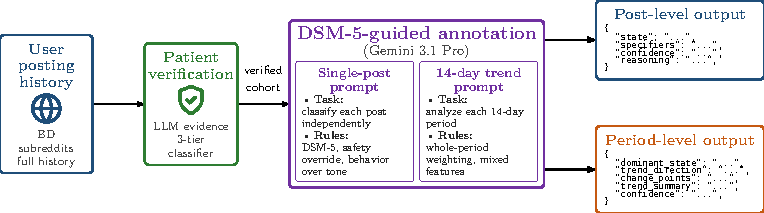
\includegraphics[width=\textwidth]{figures/fig_pipeline.pdf}
\caption{Annotation pipeline: user posting history $\rightarrow$ LLM patient verification (three-tier classifier) $\rightarrow$ DSM-5-guided annotation (Gemini 3.1 Pro) with two prompts (single-post + 14-day trend) $\rightarrow$ structured JSON outputs at the two temporal granularities.}
\label{fig:pipeline}
\end{figure}

The remainder of this section presents the annotation schema that constitutes the method's core contribution.

\subsection{Annotation Schema}
\label{sec:framework}

Our annotation schema draws on DSM-5 episode definitions~\cite{apa2013dsm5}, operationalizing them as a structured prompting framework for LLM-based annotation. The rules below were developed iteratively against an error analysis on external \del{expert} \rev{psychiatrist-guided} labels (see Sect.~\ref{sec:error}); each clinical-guidance rule named below is the schema's response to a recurring failure mode\del{ characterized there}. Because the BD-Risk data-use agreement prohibits verbatim reproduction of post text, the error analysis illustrates each pattern with a synthetic case that preserves the clinically relevant structure of the original disagreement.

\subsubsection{Post-Level State Classification}
For each individual post (submission or comment), the LLM assigns a categorical mood state from five options:

\begin{itemize}
\item \textbf{Manic:} Grandiosity, pressured writing (run-on sentences, excessive capitalization), flight of ideas (tangential topic shifts), extreme irritability or euphoria.
\item \textbf{Hypomanic:} Elevated energy and pace with maintained coherence, social disinhibition, uncharacteristic intensity without psychotic features.
\item \textbf{Depressive:} Linguistic constriction, absolutist language (\del{``never,'' ``nothing''}\rev{``never'', ``nothing''}), high self-focus (first-person pronouns), cognitive distortions, suicidal ideation.
\item \textbf{Stable:} Balanced emotional tone, metacognitive reflection, proportionate responses, community-supportive language.
\item \textbf{Uncertain:} Reserved for truly uninterpretable posts; the LLM must attempt classification before resorting to this label.
\end{itemize}

The framework also supports a \texttt{with\_mixed\_features} specifier (following DSM-5 mixed-features criteria). Before applying this specifier, the prompt requires the LLM to extract an explicit list of opposite-pole symptoms, and only assigns \texttt{with\_mixed\_features} when three or more clear opposite-pole symptoms are documented. \del{This evidence-extraction step prevents the mixed-features specifier from being used as a vague neutral label.}

\subsubsection{Period-Level Trend Analysis}
For longitudinal mood trajectory modeling, we partition each user's posting history into consecutive fixed-length periods (default: 14~days). The 14-day window length was set in consultation with clinical advisors and is grounded in DSM-5 episode-duration criteria, which define a major depressive episode as lasting at least two weeks and a manic episode as lasting at least one week~\cite{apa2013dsm5}; a 14-day window therefore captures the minimum duration of a full depressive episode and allows observation of manic-episode onset and progression. Periods are anchored at the user's first post (day 0) and advance in strict half-open intervals $[t_k, t_k + 14)$; submissions and comments are jointly assigned to the period containing their timestamp. All periods from the user's first to last post are defined; periods without posts receive a \texttt{NO\_DATA} label rather than being skipped, preserving a continuous time grid for trajectory modeling. Fig.~\ref{fig:period-slicing} illustrates the segmentation.

\begin{figure}[t]
\centering
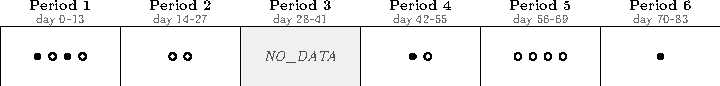
\includegraphics[width=\textwidth]{figures/fig_period_slicing.pdf}
\caption{Period segmentation (illustrative): fixed 14-day windows anchored at the user's first post (day 0). Submissions (filled circles) and comments (open circles) fall in the period containing their timestamp; empty periods (Period 3) carry the \texttt{NO\_DATA} label rather than being skipped.}
\label{fig:period-slicing}
\end{figure}

For each period containing at least one post, the LLM analyzes the collected posts \rev{(the raw submission and comment texts in the window; post-level predictions are not provided)} and produces:

\begin{itemize}
\item \textbf{Dominant state:} The primary mood state across the period (same five-class set as post-level), aggregated across the posts in the window \rev{by holistic judgment under the schema rules rather than by majority voting over post-level labels}.
\item \textbf{Trend direction:} \texttt{NO\_TREND} (state maintained), \texttt{TOWARDS\_MANIA} / \texttt{TOWARDS\_DEPRESSION} (progressive worsening toward the respective pole), or \texttt{FLUCTUATING} (alternation without a clear direction).
\item \textbf{Change points:} Specific dates or events where a mood shift occurred, with pre- and post-shift states documented.
\item \textbf{Trend summary:} A concise narrative describing the period's trajectory and the evidence supporting the dominant state.
\item \textbf{DSM-5 specifiers:} \texttt{with\_mixed\_features} when opposite-pole symptoms co-occur within the period (distinguished from sequential fluctuation).
\end{itemize}

\del{Together, the two granularities support both event-level analysis (e.g., what preceded a state change) and longitudinal trajectory modeling, with the explicit change-point fields enabling change-point detection~\cite{truong2020selective} at the textual level.}

\subsubsection{Few-Shot Example Construction}
The post-level prompt is paired with eight synthetic few-shot examples (labeled A--H), written by the authors and never drawn from BD-Risk. Each exercises a schema rule targeting a failure mode observed during development (\del{full analysis in }\rev{see} Sect.~\ref{sec:error}): A demonstrates \emph{Behavior Over Tone} on retrospective manic-side narration; B and~E demonstrate the \emph{SAFETY OVERRIDE} rule with its grandiose-mania exception; C and~D contrast \emph{Improvement-Narrative} against \emph{Whole-Post Evidence Weighting}; F counters the default-to-\emph{Uncertain} tendency on short posts; G demonstrates the \emph{Recurrent-Pattern Exception} for substance-triggered hypomania; H exercises \emph{Severity Descriptors} for \emph{Hypomanic}-vs-\emph{Stable} boundaries. Each example provides the input text with the full expected JSON output (including the \texttt{opposite\_pole\_symptoms} evidence list and reasoning), so the model observes both the target label and the evidence chain. \rev{The example count follows from this failure-mode coverage (patterns requiring contrasting demonstrations receive paired examples) rather than from tuning; we did not ablate the number of demonstrations separately.} The full prompt texts are available in the supplementary repository \rev{(see the Appendix)}.

\section{Validation Experiments}

\subsection{External Validation \protect\del{Against}\protect\rev{against} BD-Risk}
\label{sec:valid}

\subsubsection{The BD-Risk Dataset}
The BD-Risk dataset~\cite{lee2024detecting} comprises 7,346 Reddit posts from 1,025 users, each carrying a psychiatrist-guided mood level label on a 7-point scale ($-3$ to $+3$). Because the dataset recruits users via an initial MDD presentation (MDD-only and MDD$\rightarrow$BD groups), it is structurally enriched for depressive-pole content (\del{88.9\% of posts $\leq 0$ }\rev{89.0\% of posts $< 0$}).

\subsubsection{Gold State Derivation}
The BD-Risk dataset provides only ordinal mood labels; categorical states are not directly annotated. To obtain gold states for evaluation, we derive them from BD-Risk mood labels using the mapping shown in Table~\ref{tab:mapping}.

\begin{table}[t]
\caption{Mapping from BD-Risk 7-point mood labels to derived gold states.\del{ This mapping treats $+1$ as within the normal positive range (Stable) rather than pathological activation.}}
\label{tab:mapping}
\centering
\begin{tabular}{ccp{5.2cm}}
\toprule
\rev{\textbf{Mood label}} & \rev{\textbf{Gold state}} & \textbf{Notes} \\
\midrule
$-3$, $-2$, $-1$ & Depressive & \\
0, $+1$ & Stable & $+1$ = high motivation / positive mood within normal range \\
$+2$ & Hypomanic & Clear manic-side activation without psychosis \\
$+3$ & Manic & Severe manic expression with psychotic features \\
\bottomrule
\end{tabular}
\end{table}

\subsubsection{Evaluation Set Construction}
The full BD-Risk dataset exhibits a heavily skewed mood distribution (\del{88.9\% of posts $\leq 0$ }\rev{89.0\% of posts $< 0$}). Because the deployment task is BD risk detection rather than general mood classification, we deliberately oversample manic-pole posts so that per-class metrics on the underrepresented classes are computed with sufficient support.

We separate the labeled posts into two disjoint subsets. A \emph{development} subset (314 posts) is used during prompt design and failure-mode analysis. A \emph{held-out} subset (145 posts) is used exclusively for the evaluation reported below; it is \emph{author-disjoint} from the development subset, drawn by stratified sampling from BD-Risk authors not present in the development subset, with quotas ensuring sufficient per-class support across the four derived gold states (60 \emph{Depressive}, 40 \emph{Stable}, 30 \emph{Hypomanic}, 15 \emph{Manic}). All metrics in Sect.~\ref{sec:bdresult} are computed on the held-out subset; the development subset is never used to produce reported numbers. Manic-pole gold posts in BD-Risk come almost exclusively from the MDD$\rightarrow$BD group, so the held-out manic-side samples are structurally MDD$\rightarrow$BD-derived (a limitation discussed in Sect.~\ref{sec:discussion}).

\subsection{Evaluation Metrics}
\label{sec:metrics}

Throughout this paper, we refer to the \del{expert-assigned} \rev{psychiatrist-guided} labels from the BD-Risk dataset as gold labels and the LLM outputs as predictions.\del{ Gold states are derived from BD-Risk mood labels via the mapping in Table~\ref{tab:mapping}.}

We report per-class precision, recall, and F1, along with overall accuracy and macro F1, plus the confusion matrix. Two accuracy variants are reported: accuracy \emph{excluding} \emph{Uncertain} treats \emph{Uncertain} outputs as abstentions and removes them from both numerator and denominator; accuracy \emph{including} \emph{Uncertain} counts \emph{Uncertain} as incorrect, providing a conservative lower bound. Per-class precision, recall, and F1 are computed on the excluding-\rev{\emph{Uncertain}} basis.\del{ All metrics are computed on the full evaluation set.}

\subsection{Evaluation Design}
\label{sec:evaldesign}

Beyond the main BD-Risk holdout validation, we conduct three additional evaluations to characterize the schema's properties and situate its performance relative to supervised alternatives:

\begin{itemize}
\item \textbf{Zero-shot baseline comparison:} To quantify how much the structured annotation schema (DSM-5 rules, few-shot examples) contributes beyond the LLM's base capability, we re-evaluate the same model with a minimal zero-shot prompt containing only the task definition and output format.
\item \textbf{Cross-model \del{feasibility probe} \rev{portability evaluation}:} To test whether the schema generalizes beyond \del{a single LLM provider} \rev{the primary annotator}, we \del{additionally} evaluate the full schema with \del{OpenAI's GPT-5.5} \rev{five additional LLMs spanning five providers (Gemini 3.5 Flash, Claude Opus 4.8, DeepSeek V4 Pro, GLM-5.1, and GPT-5.5)}, characterizing schema portability and the impact of provider-level content-policy differences on annotation feasibility.
\item \textbf{Supervised fine-tuning baseline:} To assess whether task-specific fine-tuning with labeled data outperforms the proposed few-shot approach, we fine-tune ModernBERT-base~\cite{warner2025modernbert} on progressively larger subsets of the 314-example training pool ($n \in \{50, 100, 200, 314\}$) and evaluate on the same 145-example held-out set\del{, providing a direct comparison under identical test conditions}.
\end{itemize}

\subsection{LLM Configuration}

We use Gemini 3.1 Pro~\rev{\cite{google2026gemini31pro}} through the official API with structured JSON output\del{; the model was selected for its large context window and native structured-output generation}. Each post is processed independently with the full annotation schema and the few-shot examples described above as the system instruction; the model returns a JSON object with \texttt{state}, \texttt{opposite\_pole\_symptoms}, \texttt{specifiers}, \texttt{confidence} (High/Medium/Low), and \texttt{reasoning} fields, where \texttt{opposite\_pole\_symptoms} carries the explicit evidence list required before \texttt{with\_mixed\_features} can be assigned (see Sect.~\ref{sec:framework}). \del{For period-level annotation the LLM additionally returns \texttt{trend\_direction}, \texttt{change\_points}, and a \texttt{trend\_summary} narrative, with \texttt{confidence} on a 0--1 scale.} \rev{For period-level annotation the LLM additionally returns the period fields of Sect.~\ref{sec:framework}, with \texttt{confidence} on a 0--1 scale.} We use the Gemini 3.1 Pro default temperature of 1.0; the model is not fine-tuned.

\subsection{Validation Results}
\label{sec:bdresult}

We first validate the post-level state classification against BD-Risk \del{expert} \rev{psychiatrist-guided} labels (Table~\ref{tab:state-metrics}: per-class metrics with macro-aggregated summary).

\begin{table}[t]
\caption{Per-class metrics with macro summary on the held-out subset (\rev{$n=145$}; 138 excluding 7 \emph{Uncertain}). Accuracy excl./incl. \emph{Uncertain} = 65.9\% / 62.8\%; macro F1 is the primary metric because the subset is intentionally stratified. \rev{Bootstrap 95\% confidence intervals (1{,}000 resamples): macro F1 [0.430, 0.610]; \emph{Manic} F1 [0.000, 0.348].}}
\label{tab:state-metrics}
\centering
\setlength{\tabcolsep}{9pt}
\begin{tabular}{lrrrr}
\toprule
\textbf{State} & \textbf{Precision} & \textbf{Recall} & \textbf{F1} & \textbf{Support} \\
\midrule
Depressive & 0.630 & \textbf{0.879} & \textbf{0.734} & 58 \\
Stable & 0.659 & 0.784 & 0.716 & 37 \\
Hypomanic & \textbf{0.833} & 0.357 & 0.500 & 28 \\
Manic & \textbf{1.000} & 0.067 & 0.125 & 15 \\
\midrule
\emph{Macro avg} & \emph{0.781} & \emph{0.522} & \emph{0.519} & \emph{138} \\
\bottomrule
\end{tabular}
\end{table}

\emph{Depressive} recall is high (87.9\%) and \emph{Stable} recall is moderate (78.4\%), while \emph{Hypomanic} and \emph{Manic} recall remain low (35.7\% and 6.7\%), indicating that the LLM correctly recognizes most depressive and stable posts while missing a majority of manic-pole cases. The confusion matrix (Table~\ref{tab:state-cm}) makes the dominant error flow explicit: among the 30 gold-\emph{Hypomanic} posts, 12 are predicted as \emph{Depressive} and 6 as \emph{Stable}; among the 15 gold-\emph{Manic} posts, 11 are predicted as \emph{Depressive} and 2 as \emph{Stable}. The Manic-to-Depressive error flow is a recurring pattern with a likely label-text origin that we discuss in Sect.~\ref{sec:discussion}.

\begin{table}[t]
\caption{State confusion matrix on the held-out subset (rows: derived gold state; columns: LLM prediction). DEP = \rev{\emph{Depressive}}, STA = \rev{\emph{Stable}}, HYP = \rev{\emph{Hypomanic}}, MAN = \rev{\emph{Manic}}, UNC = \rev{\emph{Uncertain}}.}
\label{tab:state-cm}
\centering
\setlength{\tabcolsep}{8pt}
\begin{tabular}{lrrrrrr}
\toprule
\cmpredheader
\textbf{Gold} & \textbf{DEP} & \textbf{STA} & \textbf{HYP} & \textbf{MAN} & \textbf{UNC} & \textbf{Total} \\
\midrule
Depressive & \textbf{51} & 7 & 0 & 0 & 2 & 60 \\
Stable & 7 & \textbf{29} & 1 & 0 & 3 & 40 \\
Hypomanic & 12 & 6 & \textbf{10} & 0 & 2 & 30 \\
Manic & 11 & 2 & 1 & \textbf{1} & 0 & 15 \\
\bottomrule
\end{tabular}
\end{table}

These \emph{Hypomanic} errors are concentrated on gold $+2$ posts whose manic-side activation is masked by negative tone, a pattern that the current prompt does not fully resolve.

\subsection{Supervised Fine-Tuning Baseline}
\label{sec:bert}

To contextualize the few-shot LLM results, we compare against a supervised baseline. We fine-tune ModernBERT-base~\cite{warner2025modernbert} (149M parameters) on the same BD-Risk training pool using progressively larger labeled subsets ($n \in \{50, 100, 200, 314\}$), evaluating on the identical 145-example held-out set. Each tier is trained for 10 epochs with a learning rate of $2 \times 10^{-5}$ and a maximum sequence length of 2,048 tokens; for tiers 50--200, we report the mean and standard deviation over five random training-set samples (seeds 42--46), while tier 314 uses all available training examples and reports variance over five random initializations. Table~\ref{tab:bert-baseline} summarizes the results alongside the LLM conditions.

\begin{table}[t]
\caption{Supervised fine-tuning baseline vs.~LLM annotation on the held-out subset ($n = 145$). ModernBERT results report mean $\pm$ std over \del{5} \rev{five} seeds. The few-shot LLM uses eight synthetic examples and requires no labeled training data \rev{at inference time}.}
\label{tab:bert-baseline}
\centering
\setlength{\tabcolsep}{7pt}
\begin{tabular}{llrr}
\toprule
\textbf{Method} & \textbf{Training data} & \textbf{Macro F1} & \textbf{$\Delta$ vs.~few-shot} \\
\midrule
ModernBERT & $n = 50$ & $0.306 \pm 0.022$ & $-0.213$ \\
ModernBERT & $n = 100$ & $0.337 \pm 0.018$ & $-0.182$ \\
ModernBERT & $n = 200$ & $0.372 \pm 0.019$ & $-0.147$ \\
ModernBERT & $n = 314$ & $0.398 \pm 0.018$ & $-0.121$ \\
\midrule
Gemini 3.1 Pro & zero-shot & $0.459$ & $-0.060$ \\
Gemini 3.1 Pro & 8 few-shot & $\mathbf{0.519}$ & --- \\
\bottomrule
\end{tabular}
\end{table}

ModernBERT macro F1 increases monotonically with training size (0.306 $\rightarrow$ 0.398), yet even at the maximum available training size ($n = 314$), it falls short of Gemini few-shot (0.519) by 0.121 and barely approaches the Gemini zero-shot level (0.459). We additionally explored training for 15 and 20 epochs on the full 314-example set; the best configuration (15 epochs: $0.454 \pm 0.038$) narrows the gap yet remains below the few-shot result.

Per-class analysis reveals that ModernBERT shares the same manic-pole difficulty observed in the LLM results (Sect.~\ref{sec:bdresult}): across the five tier-314 runs, \emph{Manic} recall averages 0.04 (2 of 5 runs produce zero \emph{Manic} recall), while \emph{Depressive} and \emph{Stable} F1 average 0.51 and 0.62 respectively. This parallel suggests that the manic-pole limitation is rooted in the BD-Risk \del{label--text} \rev{label-text} relationship \del{(Sect.~\ref{sec:error}, Pattern~1)} \rev{(Sect.~\ref{sec:discussion})} rather than in the choice of model architecture.

\del{From a practical standpoint, constructing 314 expert-labeled training examples for BD mood-state classification requires psychiatric expertise and substantial annotation effort. The few-shot LLM approach achieves higher performance} \rev{From a practical standpoint, the few-shot approach outperforms the supervised baseline} using only eight synthetic examples embedded in the prompt, with no manual labeling \rev{at inference time; schema development, in turn, drew on the 314-post development subset for error analysis (Sect.~\ref{sec:valid})}. \del{This comparison supports the proposed method's practical advantage in low-resource clinical NLP settings where labeled data is scarce.} \rev{This supports the method's practical advantage in low-resource clinical NLP settings, where labeled data is scarce and annotation requires psychiatric expertise.}

\subsection{Interpretation of Validation Results}

\subsubsection{The Uncertain Label as Quality Control}
The LLM assigned \emph{Uncertain} to 7 posts (4.8\%), abstaining when post content was insufficient for state assessment, consistent with the prompt's explicit instruction to prefer abstention over forced classification. \emph{Uncertain} emissions are distributed across gold classes\del{ (2 \emph{Depressive}, 3 \emph{Stable}, 2 \emph{Hypomanic}, 0 \emph{Manic})}, with no strong concentration on a single pole.

\subsubsection{Schema Contribution: Comparison with a Zero-Shot Baseline}
Following the design in Sect.~\ref{sec:evaldesign}, we compare the full schema against a minimal zero-shot prompt on the held-out subset. \rev{This comparison constitutes an ablation of the schema in its entirety; finer-grained per-rule ablations are left for future work.} The zero-shot prompt retains only the task definition (post $\rightarrow$ one of five states) and the output JSON fields; all DSM-5 rules, \emph{SAFETY OVERRIDE}, \emph{Severity Descriptors}, and few-shot examples are removed. Table~\ref{tab:zeroshot} reports the side-by-side metrics.

\begin{table}[t]
\caption{Schema contribution on the held-out subset (\rev{$n=145$}). Both runs use Gemini 3.1 Pro with the same JSON output; the only variable is the system prompt (zero-shot: task definition only; full schema: \emph{SAFETY OVERRIDE}, \emph{Severity Descriptors}, \emph{Clinical Guidance}, eight few-shot examples).}
\label{tab:zeroshot}
\centering
\setlength{\tabcolsep}{8pt}
\begin{tabular}{lrrr}
\toprule
\textbf{Metric} & \textbf{Zero-shot} & \textbf{Full schema} & \textbf{$\Delta$} \\
\midrule
Accuracy (incl.\ Uncertain) & 51.7\% & \textbf{62.8\%} & $+$11.1 pp \\
Accuracy (excl.\ Uncertain) & 63.6\% & \del{65.9\%} \rev{\textbf{65.9\%}} & $+$2.3 pp \\
Macro F1 & 0.459 & \textbf{0.519} & $+$0.060 \\
Uncertain count & 27 & \textbf{7} & $-$20 \\
\zsperclassrows
\bottomrule
\end{tabular}
\end{table}

Three observations frame the schema's value. First, the largest single effect is a $4\times$ reduction in \emph{Uncertain} emissions (27 $\rightarrow$ 7): the structured schema gives the LLM the vocabulary to commit to a label rather than abstain, which explains why the accuracy gain including \emph{Uncertain} (+11.1 pp) is much larger than the gain excluding \emph{Uncertain} (+2.3 pp). Second, \emph{Stable} classification \del{benefits the most in per-class F1 (+0.116)} \rev{gains +0.116 in per-class F1}, driven by the \rev{\emph{Severity Descriptors}'} explicit ``Stable includes mild positive activation'' rule that prevents the LLM from defaulting non-pathological positive posts to \emph{Depressive} or \emph{Uncertain}. \del{Third, \emph{Depressive} and \emph{Hypomanic} F1 are unchanged, suggesting that the full schema did not materially alter performance for those categories on this subset, and \emph{Manic} remains poorly recalled in both runs (0/15 zero-shot vs.~1/15 schema, counting \emph{Uncertain} as incorrect), further suggesting that the manic-pole limitation is structural (label-text consistency, Sect.~\ref{sec:discussion}) rather than a limitation resolved by this richer prompt.} \rev{Third, \emph{Depressive} and \emph{Hypomanic} F1 are unchanged, and \emph{Manic} remains poorly recalled in both runs (F1 0.000 vs.~0.125); the Discussion (Sect.~\ref{sec:discussion}) attributes this manic-pole floor to the label-text consistency issue rather than to prompt design.}

The comparison suggests that the schema's primary contribution is coverage and decisiveness (preventing abstention, anchoring border-class decisions) rather than raw classification accuracy on the cases the LLM is already confident about.

\subsubsection{Cross-Model \del{Annotation Feasibility} \rev{Schema Portability}}
\label{sec:crossmodel}
\del{As a cross-model probe (Section 4.3), we evaluated the full schema with OpenAI's GPT-5.5 (\texttt{reasoning\_effort} = \texttt{"high"}) on the same 145 held-out posts. The schema and JSON output format were identical to the main run; only the underlying model changed.} \rev{Following the design in Sect.~\ref{sec:evaldesign}, Table~\ref{tab:crossmodel} reports the four additional LLMs with complete annotations on the held-out subset; GPT-5.5, which declined a majority of posts, is reported in the text.}

\begin{table}[t]\revfloat
\caption{Cross-model evaluation on the held-out subset ($n = 145$), identical 8-example few-shot prompt. Macro F1 is over the four target classes, excluding \emph{Uncertain} (see Sect.~\ref{sec:bdresult}). Dep/Hyp/Man Rec = recall for the \emph{Depressive}/\emph{Hypomanic}/\emph{Manic} classes; Unc = number of \emph{Uncertain} outputs.}
\label{tab:crossmodel}
\centering
\setlength{\tabcolsep}{5pt}
\begin{tabular}{lrrrrr}
\toprule
\textbf{Model} & \textbf{Macro F1} & \textbf{Dep Rec} & \textbf{Hyp Rec} & \textbf{Man Rec} & \textbf{Unc} \\
\midrule
Gemini 3.5 Flash & $\mathbf{0.564}$ & $0.850$ & $0.379$ & $0.200$ & 3 \\
Gemini 3.1 Pro & $0.519$ & $0.879$ & $0.357$ & $0.067$ & 7 \\
Claude Opus 4.8 & $0.535$ & $0.932$ & $0.429$ & $0.067$ & 7 \\
GLM-5.1 & $0.456$ & $0.881$ & $0.286$ & $0.000$ & 4 \\
DeepSeek V4 Pro & $0.432$ & $0.833$ & $0.241$ & $0.000$ & 2 \\
\bottomrule
\end{tabular}
\end{table}

\rev{All five models in Table~\ref{tab:crossmodel} complete the annotation for every post with zero refusals, indicating the schema is not provider-specific. Manic-pole underdetection persists across model families, reinforcing the structural interpretation (Sect.~\ref{sec:discussion}) that the difficulty stems from the BD-Risk label-text relationship rather than from any single model.}

\rev{Because the corpus was annotated with Gemini 3.1 Pro prior to this comparison, the existing annotations remain unchanged; re-annotation with a stronger model remains future work.}

GPT-5.5 \rev{(evaluated with \texttt{reasoning\_effort} = \texttt{"high"})} declined to classify 103 of 145 held-out posts (71.0\%) with a \del{verbatim }refusal\del{ (\texttt{"I'm sorry, but I cannot assist with that request."})}, concentrated on posts containing explicit self-harm or suicidal content, the safety-relevant subset that BD-Risk includes by clinical design and that the \emph{SAFETY OVERRIDE} rule is built to handle. The prompt's clinical-research framing did not overcome the refusal. \del{Gemini 3.1 Pro produced structured output for all 145 posts under the same prompt.} On the 42 posts GPT-5.5 did classify (skewed away from depressive-crisis content\del{: 16 \emph{Depressive}, 10 \emph{Stable}, 12 \emph{Hypomanic}, 4 \emph{Manic}}), it achieved macro F1 of 0.710 (Gemini \rev{3.1 Pro on the same 42 posts}: 0.649), driven primarily by higher \emph{Manic} recall\del{ (2/4 vs.~1/4)}. \del{The schema produces sensible structured output, suggesting it is not inherently Gemini-specific. However, the} \rev{The} subset selection is the dominant effect: GPT-5.5 systematically filtered out the hard depressive-crisis posts that drive most of Gemini's error rate\del{ on the full held-out subset}, so the macro-F1 comparison overstates GPT-5.5's effective competence. \del{Most importantly, a} \rev{A 71.0\%} refusal rate renders GPT-5.5 infeasible as a stand-alone annotator for psychiatric corpora regardless of intrinsic capability.

\subsubsection{Error Analysis}
\label{sec:error}
We characterize six failure modes identified through manual analysis of LLM-vs-BD-Risk disagreements on the development subset. For each pattern, we name the schema rule designed to mitigate it and note whether the rule resolves the pattern on the held-out subset or whether it remains a residual error. Manic-pole posts misclassified as depressive or stable remain the dominant residual failure mode (quantified in Sect.~\ref{sec:bdresult}).

Pattern 1\rev{, the dominant manic-side error, is the LLM ignoring retrospective behavioral cues}. \dnote{Pattern 1--6：見出し形式を本文の文章に書き換え（内容は変更なし）} When users describe manic-episode behaviors\del{ (impulsive spending, aggressive confrontations, hyperactivity)} in a retrospective post written with remorse or self-blame, the LLM anchors on the current emotional tone rather than the clinical significance of the described behaviors\del{, and predicts \emph{Depressive}}. The schema's \emph{Behavior Over Tone} rule is designed to address this conflation; however, \del{it} \rev{the pattern} remains the dominant residual error on the held-out subset\del{, indicating that the rule reduces the pattern without fully eliminating it}. \emph{Synthetic case:} a user recounts a week of reckless spending and impulsive decisions in a tone of deep regret and self-condemnation; gold is \emph{Hypomanic} (the behaviors are hallmark manic symptoms), the LLM predicts \emph{Depressive} (anchored on the self-deprecating tone).

Pattern 2 \rev{is the conflation of mixed features with neutrality}. When a post carries symptoms from both poles simultaneously\del{ (e.g., severe sleep disruption and inability to concentrate alongside aggressive outbursts)}, the LLM sometimes treats the coexistence as cancellation\del{ and defaults to \emph{Stable}}. Under DSM-5~\cite{apa2013dsm5}, mixed features should instead surface as a \texttt{with\_mixed\_features} specifier on the dominant pole. The schema's mixed-features rules reduce this conflation, though residual instances remain when symptom signals are subtle. \emph{Synthetic case:} a user writes that they have not slept in three days, cannot focus at work, and snapped at their partner, all in the same post; gold is \emph{Hypomanic} with mixed features (decreased need for sleep alongside dysphoric irritability), the LLM predicts \emph{Stable} on the reasoning that the signals ``balance out''.

Pattern 3\rev{, a safety-critical case, is calm writing style masking suicidal ideation}. Some posts express suicidal ideation (``I want to die'') in calm\del{, reflective, or educational} prose; the LLM reads the linguistic register as stable\del{ and classifies accordingly}, while the gold state is \emph{Depressive} ($-3$). \del{Calm writing does not rule out suicidal crisis, and the} \rev{The} schema's explicit \emph{SAFETY OVERRIDE} rule forces \emph{Depressive} whenever crisis-level language is present regardless of surrounding tone. On the held-out subset, no \emph{Stable} or \emph{Uncertain} predictions were observed for posts with explicit suicidal content\del{, suggesting that the rule addresses this pattern on the evaluated subset}. \emph{Synthetic case:} a user posts a coherent essay about public misconceptions of depression; embedded in the second paragraph, in the same calm register, is a single sentence noting that the writer quietly thinks about not waking up most mornings.

Pattern 4 \rev{is end-of-post hope overriding pervasive impairment}. Posts describing severe functional impairment\del{ (academic collapse, inability to maintain daily routines, social withdrawal)} sometimes close with a single hopeful sentence\del{ (e.g., ``my therapist said maybe I shouldn't give up'')}, and the LLM anchors on this terminal positive signal (consistent with a recency bias)\del{ to predict \emph{Stable} while the gold label tracks the pervasive impairment throughout}. The schema's \emph{Whole-Post Evidence Weighting} rule addresses this\del{ by instructing the LLM to weigh the dominant clinical picture over terminal sentiment}; the zero-shot comparison \del{(Table~\ref{tab:zeroshot}) }shows that the full schema improves \emph{Stable} F1 by +0.116, consistent with reduced over-assignment of \emph{Stable} to impaired posts. \emph{Synthetic case:} a user reports missing every class for a month, eating almost nothing this week, and losing the ability to reply to friends, closing with ``maybe tomorrow will be different''; gold is \emph{Depressive} on the pervasive impairment, the LLM predicts \emph{Stable}.

Pattern 5 \rev{concerns substance-induced activation versus endogenous mood}. When users describe mood elevation explicitly attributed to substances\del{ (e.g., caffeine-induced euphoria described as feeling ``on top of the world'')}, the LLM may interpret \del{these cues} \rev{the elevation} as hypomanic mood\del{, while gold labels distinguish acute pharmacological activation from endogenous baseline}. The schema's \emph{Substance vs.~Endogenous Mood} rule addresses this boundary and also covers the \emph{Recurrent-Pattern Exception} where an unusual reactivity to a common substance is itself bipolar-spectrum. This pattern is rare in the held-out subset\del{; the rule's primary effect is preventing false \emph{Hypomanic} predictions on substance-attributed posts}. \emph{Synthetic case:} a user writes that after a fourth coffee they suddenly feel ``unbeatable and ready to overhaul'' their apartment, attributing the surge to caffeine and expecting an evening crash; gold is \emph{Stable} (acute, externally caused, self-labeled), the LLM predicts \emph{Hypomanic} on the surface cues.

Pattern 6 \rev{is \emph{Uncertain} masking embedded clinical signals}. \emph{Uncertain} functions appropriately in the large majority of cases\del{; the failure described here is rare}. \del{The LLM correctly identifies the post as metacommentary or informational, then fails to surface clinically significant content embedded inside.} \emph{Synthetic case:} a user writes a meta-commentary criticizing how recovery is portrayed online and, mid-argument, notes parenthetically that they have been thinking about ending things; gold is \emph{Depressive}, the LLM defaults to \emph{Uncertain} on the meta-discussion register. The \emph{SAFETY OVERRIDE} rule mitigates this pattern\del{ by forcing \emph{Depressive} on crisis-level language regardless of overall framing} \rev{and appears effective on the held-out subset}. \del{Like Pattern 3, the rule appears effective on the held-out subset: no crisis-level posts were classified as \emph{Uncertain}.}

\section{Longitudinal Demonstration: Period-Level Mood Trends}
\label{sec:pilot}

We continuously crawl three BD-focused subreddits (r/bipolar, r/BipolarReddit, r/bipolar2) via the Reddit API, retrieving each active author's full posting history (submissions and comments) with periodic re-crawls to capture ongoing activity. Posting to a mental-health-related subreddit is a necessary yet insufficient signal of a BD diagnosis: many such posts come from clinicians, family members, or general community participants. To screen the candidate pool, we apply an LLM three-tier classifier (Gemini 3.1 Pro, separate prompt) that scans each author's full posting history and returns \texttt{verified} (explicit first-person diagnostic statements, e.g., ``I was diagnosed with bipolar II in 2019'', or specific treatment/hospitalization narratives), \texttt{probable} (consistent self-identification through symptoms, medication, or community-membership tone without an explicit diagnosis statement), or \texttt{unverified} (no diagnostic signal). Only the \texttt{verified} and \texttt{probable} tiers are admitted to the annotation cohort; this matches the inclusion model used in prior BD social-media datasets~\cite{jagfeld2021understanding,sekulic2018not} with stricter per-user evidence gating than a one-post membership rule. After this verification, the \rev{\texttt{verified}+\texttt{probable}} cohort comprises 115 of 124 candidate authors. Users with fewer than two 14-day periods containing posts (i.e., insufficient longitudinal span for trend analysis) are excluded. The remaining 105 users contribute 2,611 submissions and 12,812 comments spanning April 2019 through May 2026, yielding 1,794 valid analysis periods. \rev{Across the 105 users, the continuous 14-day grids comprise 4,091 windows in total, of which 1,794 contain at least one post and the remaining 2,297 carry the \texttt{NO\_DATA} label; non-empty windows contain a median of 3 posts (submissions and comments; interquartile range 1--9). Because no period-level expert ground truth exists, the analysis in this section is exploratory.}

\begin{figure}[t]
\centering
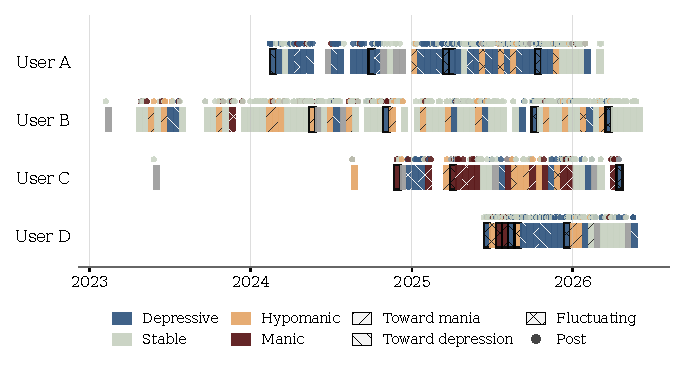
\includegraphics[width=\textwidth]{figures/fig_timeline.pdf}
\caption{Mood trajectories for four anonymized users (A: depressive with fluctuation\del{, 49 periods}; B: hypomanic-leaning with frequent manic transitions\del{, 74 periods}; C: manic-dominant with \del{rapid cycling} \rev{a pattern consistent with rapid cycling}\del{, 36 periods}; D: dense posting with high mixed-features incidence\del{, 25 periods}). Bars = 14-day periods (color = dominant state; hatch = trend direction; thin black border = \texttt{with\_mixed\_features}); dots above bars = post-level annotations, color-coded by post state.}
\label{fig:user-timeline}
\end{figure}

Most 14-day windows show \texttt{NO\_TREND} \rev{(Table~\ref{tab:pilot-dists})}, as expected: DSM-5 episode-duration criteria require $\geq$1 week for mania, $\geq$4 days for hypomania, and $\geq$2 weeks for major depression~\cite{apa2013dsm5}, and untreated episodes typically last weeks to months, so within-window transitions are infrequent; the rare \texttt{TOWARDS\_DEPRESSION} and \texttt{TOWARDS\_MANIA} trends \rev{may} mark episode onset or escalation, the signals most relevant for early intervention. \emph{Stable} and \emph{Depressive} states dominate (42.6\% and 31.4\% of periods), while manic-pole states constitute a smaller share (\emph{Hypomanic} 8.8\%, \emph{Manic} 3.0\%), broadly consistent with the depressive-pole predominance reported in long-term BD cohort studies~\cite{grande2016bipolar} while reflecting the selection and posting biases of Reddit communities.

\begin{table}[t]
\caption{Period-level distributions on the 105-user cohort ($n = 1{,}794$). Left: trend directions\del{ (\texttt{NO\_TREND} = state maintained, \texttt{FLUCTUATING} = alternation, \texttt{TOWARDS\_MANIA} / \texttt{TOWARDS\_DEPRESSION} = worsening)}. Right: dominant states; \texttt{with\_mixed\_features} was applied to 84 periods (4.7\%).}
\label{tab:pilot-dists}
\centering
\begin{tabular}{lrr}
\toprule
\textbf{Trend direction} & \textbf{Periods} & \textbf{\%} \\
\midrule
\rev{\texttt{NO\_TREND}} & 1,506 & 83.9\% \\
\rev{\texttt{FLUCTUATING}} & 106 & 5.9\% \\
\rev{\texttt{TOWARDS\_DEPRESSION}} & 105 & 5.9\% \\
\rev{\texttt{TOWARDS\_MANIA}} & 77 & 4.3\% \\
\bottomrule
\end{tabular}
\hspace{2em}
\begin{tabular}{lrr}
\toprule
\textbf{Dominant state} & \textbf{Periods} & \textbf{\%} \\
\midrule
Stable & 765 & 42.6\% \\
Depressive & 564 & 31.4\% \\
Hypomanic & 157 & 8.8\% \\
Manic & 54 & 3.0\% \\
Uncertain & 254 & 14.2\% \\
\bottomrule
\end{tabular}
\end{table}

Table~\ref{tab:post-state-dist} breaks the post-level assignments down by content type; the \del{submission--comment} \rev{submission-comment} asymmetry and its implications are discussed in Sect.~\ref{sec:discussion}. The \emph{Uncertain} rate is low for both content types ($\leq$3.0\%), reflecting the model's confidence on the corpus.

\begin{table}[t]
\caption{Post-level state distribution across the 105-user cohort, separated by content type \rev{(submissions $n = 2{,}611$; comments $n = 12{,}812$)}.\del{ Posts (submissions, $n = 2{,}611$) function as longer-form emotional disclosures and carry the majority of polar-state labels; comments ($n = 12{,}812$) are predominantly conversational replies labeled \emph{Stable}.}}
\label{tab:post-state-dist}
\centering
\setlength{\tabcolsep}{8pt}
\begin{tabular}{lrrrr}
\toprule
\textbf{State} & \textbf{Posts} & \textbf{\%} & \textbf{Comments} & \textbf{\%} \\
\midrule
Manic & 98 & 3.8\% & 93 & 0.7\% \\
Hypomanic & 277 & 10.6\% & 292 & 2.3\% \\
Stable & 1,217 & 46.6\% & 11,287 & 88.1\% \\
Depressive & 961 & 36.8\% & 755 & 5.9\% \\
Uncertain & 58 & 2.2\% & 385 & 3.0\% \\
\bottomrule
\end{tabular}
\end{table}

The trajectory data adds a temporal dimension that per-post or per-user classification cannot provide\del{: prior approaches yield static snapshots (a single diagnostic label or an isolated mood score) without capturing how states transition over weeks to months}. Fig.~\ref{fig:user-timeline} illustrates individual-level patterns that this temporal view reveals: User~B exhibits a sequence of hypomanic periods followed by manic escalation, \del{indicative of} \rev{a pattern consistent with} episode onset; User~D shows frequent mixed-features periods\del{, consistent with a rapid-cycling presentation}\rev{; User~C shows a pattern consistent with rapid cycling}. These trajectory-level signals (episode onset, escalation, and cycling patterns) cannot be recovered from per-post labels in isolation\del{ and represent the type of information that could inform clinical early-warning systems or patient self-monitoring tools, although their clinical utility remains to be validated with expert-annotated period-level ground truth}\rev{; we present them as unvalidated hypotheses that could, once confirmed against expert-annotated period-level ground truth, inform clinical early-warning systems or patient self-monitoring tools}.

\section{Discussion}
\label{sec:discussion}

Prior BD datasets primarily provide per-user labels~\cite{cohan2018smhd,sekulic2018not} or per-post scores~\cite{lee2024detecting}, leaving period-level mood trajectories underrepresented; our period-level annotations add this dimension by recording in each 14-day window the dominant state, the trend direction (whether mood is shifting), and change points (when shifts occur). From the trend distribution (Sect.~\ref{sec:pilot}), four \rev{exploratory} observations stand out. (1) \texttt{TOWARDS\_MANIA} and \texttt{TOWARDS\_DEPRESSION} trends are rare yet among the most clinically significant signals, as they \rev{may} mark episode onset where intervention has the most impact. (2) \texttt{FLUCTUATING} periods may correspond to rapid cycling or mixed presentations that single-post labels cannot capture. (3) Post-level states and period-level trends together enable hierarchical modeling\del{: predicting the next period's trajectory from the sequence of post-level features}. (4) The dominant-state distribution preserves meaningful manic-pole representation, in contrast to MDD-recruited cohorts (BD-Risk: \del{88.9\% depressive-or-neutral} \rev{89.0\% depressive-pole}); this balance matters for downstream models that must distinguish manic-pole from depressive states. The trend distributions are broadly consistent with clinical expectations for BD-related online discussion\rev{~\cite{apa2013dsm5,grande2016bipolar}}; direct external validation would require period-level expert annotations. A complementary direction is to model the absence signal in \texttt{NO\_DATA} periods: reduced posting is sometimes associated with depression in digital-phenotyping research~\cite{faurholt2018smartphone}, yet the relationship is heterogeneous, so absence modeling would require posting-frequency baselines beyond a text-based pipeline.

Table~\ref{tab:post-state-dist} also reveals a sharp \del{submission--comment} \rev{submission-comment} asymmetry: 51.2\% of submissions carry a polar state vs.~\del{9.1\%} \rev{8.9\%} of comments, which are dominated by \emph{Stable} (88.1\%). Submissions are longer-form disclosures while comments are short replies. Two downstream implications: a per-post classifier on a comment-heavy corpus is likely to appear over-confident on \emph{Stable}, so per-content-type metrics are preferable to a single aggregate; and trajectory models should either up-weight submissions or rely on the period-level dominant-state annotation\del{ (which already aggregates across content types within the window)} as the primary trajectory signal. \rev{This asymmetry also explains the apparent amplification from 16.1\% polar labels at the item level to 43.2\% polar-dominant periods: dominant-state assignment is a holistic judgment over the window rather than proportional voting, and 93.8\% of the 775 polar-dominant periods contain at least one same-pole post-level label. The median such period holds five posts (submissions and comments), so a few polar submissions typically determine the dominant state against a \emph{Stable}-dominated comment background.}

A pronounced manic-pole recall gap persists: the LLM achieves 87.9\% recall for \emph{Depressive} yet only 35.7\% for \emph{Hypomanic} and 6.7\% for \emph{Manic} on the held-out subset. Two factors compound this asymmetry. First, a model property: depressive language has stereotypical surface markers (negativity, self-focus, hopelessness), while manic-pole states often manifest through \emph{described behaviors} (spending sprees, reduced sleep need, grandiose plans) narrated in any tone, and the LLM reads tone rather than the clinical significance of the behaviors described (see Pattern~1 in Sect.~\ref{sec:error}). Second, a \del{label--text} \rev{label-text} consistency issue in the BD-Risk annotation rule: as specified by~\cite{lee2024detecting} (Section~3.2), ``posts exhibiting both manic and depressive moods are regarded as manic moods'', an asymmetric tie-breaker that elevates any mixed manic+depressive post to the manic side. Combined with the dataset's MDD$\rightarrow$BD recruitment, this yields gold-label \emph{Manic} ($+3$) posts whose textual content matches BD-Risk's own definition of $-3$ (``extreme anxiety and having suicidal thoughts''). A single-post LLM applying clinical-safety priors (classifying explicit self-harm content as \emph{Depressive}) will systematically underperform on these posts, since the only signal it has is the very content the labeling rule overrode. \rev{The cross-model evaluation (Sect.~\ref{sec:crossmodel}) provides direct evidence for the structural interpretation: \emph{Manic} recall remains low across the LLMs in Table~\ref{tab:crossmodel} and for the supervised ModernBERT baseline (Sect.~\ref{sec:bert}); all architectures converge on the same manic-pole floor.} The Manic-recall ceiling\del{ of 6.7\%} in Table~\ref{tab:state-metrics} thus reflects a structural mismatch, not solely a model limitation (downstream implications in Limitations).

\section{Limitations}

The proposed method and corpus are subject to \del{constraints that we group into evaluation scope, gold-state derivation, manic-pole interpretability, cohort framing, and release-time reliability} \rev{the following constraints}.

Regarding evaluation scope, \del{the main BD-Risk validation uses a single annotator (Gemini 3.1 Pro); a complementary GPT-5.5 probe (macro F1 0.710 on 42 non-refused posts) suggests that the schema is not inherently Gemini-specific, yet OpenAI's current content policy prevents scale-up (\del{71\% }\rev{71.0\%} refusal on the held-out subset), so the per-class numbers on the 145-post held-out subset should be read as Gemini-specific} \rev{the cross-model evaluation (Sect.~\ref{sec:crossmodel}) confirms schema portability across the four additional LLMs that completed the full 145-post holdout (macro F1 0.432--0.564; the fifth, GPT-5.5, declined a majority of posts), yet the corpus itself was annotated exclusively with Gemini 3.1 Pro; per-class reliability estimates thus remain Gemini-specific}. The quantitative validation is also at the post level only, because few per-post expert-labeled BD datasets at sufficient scale are available for research use\del{ (BD-Risk was obtained through a formal data request and ethics review, and comparable shared-task corpora face similar access barriers)}; period-level trends, a key contribution of the method, are not externally validated. \rev{The schema is developed and validated on English-language Reddit data under DSM-5 criteria; transfer to other languages, platforms, or clinical domains would require prompt adaptation and re-validation, which this study does not test. Period-level results are additionally conditioned on the 14-day window length and the first-post anchor (Sect.~\ref{sec:framework}); alternative window lengths (e.g., 7 or 30 days) and shifted anchors would require re-annotating the corpus and remain future work.}

For gold-state derivation, the categorical states used as ground truth are derived from BD-Risk mood labels via a deterministic mapping (Table~\ref{tab:mapping}) rather than being directly annotated by experts as categorical states. This mapping introduces imprecision: the boundary between adjacent categories is inherently uncertain (e.g., BD-Risk mood label $+1$ may reflect mild hypomania rather than stable mood), and the ordinal intensity score does not always correspond to a categorical clinical judgment\del{ (e.g., a recovery narrative within an ongoing depressive episode may receive a neutral mood score while remaining clinically depressive)}. \del{Inter-expert agreement} \rev{Agreement among the two experts and the researcher annotators on a 150-post validation subset} (Krippendorff's $\alpha = 0.87$\rev{; expert-expert Cohen's $\kappa = 0.69$}) is measured at the ordinal level, and mapping to categorical states amplifies disagreement at boundaries. \rev{Because the released data do not identify the validated subset, whether any of the 145 held-out posts fall within the 150 expert-validated posts (2.0\% of the dataset, drawn from 120 users) cannot be established.} Consequently, some apparent misclassifications may reflect mapping artifacts, and the reported accuracy figures should be interpreted as lower bounds on the schema's true reliability.

Regarding manic-pole interpretability, two factors limit how the \del{Manic-pole} \rev{manic-pole} numbers can be read. First, the held-out \emph{Manic} class is small ($n=15$, because the entire BD-Risk dataset contains only 28 mood-$+3$ posts); the \rev{bootstrap} 95\% confidence interval around the \del{Manic-F1} \rev{\emph{Manic} F1} estimate is wide (\del{$\pm$ approximately 13 percentage points }\rev{[0.000, 0.348] over 1{,}000 resamples}), and small \del{Manic-F1} \rev{\emph{Manic} F1} differences should not be interpreted as significant. Second, the Manic-recall ceiling of 6.7\% is bounded by a structural mismatch between BD-Risk's asymmetric tie-breaking rule and the textual evidence available to a per-post classifier (full analysis in Sect.~\ref{sec:discussion}); recovering label-text consistency would require either re-annotation under text-only criteria or a longitudinal evaluation protocol that supplies the temporal context the annotators had access to.

For cohort framing, patient verification is LLM-based and screens for self-disclosure of a BD diagnosis in the user's posting history; it does not constitute clinical confirmation. \del{This follows the inclusion model used in prior BD social-media datasets~\cite{jagfeld2021understanding,sekulic2018not} with stricter per-user evidence gating than a one-post membership rule.} Some users in the \texttt{verified} or \texttt{probable} tiers may describe a BD diagnosis without one having been clinically established, and the cohort conversely excludes users with BD who never disclose the diagnosis publicly. \del{Reddit is also a self-selected, asynchronous channel, so the relationship between its posts and clinically observed mood states requires further investigation.} Downstream uses that require clinician-confirmed BD status should treat the cohort as an LLM-screened self-identified sample rather than a clinical cohort.

Regarding release-time reliability, all period-level (1,794) and post-level (15,423) annotations are produced entirely by the LLM; we have not yet conducted manual spot-checking on a stratified sample across mood states, confidence levels, and trend directions. The held-out validation suggests stronger reliability for \emph{Depressive} labels\del{ (87.9\% recall, 73.4\% F1)} than for manic-pole labels; \emph{Hypomanic} labels have moderate reliability\del{ (35.7\% recall, 50.0\% F1)} with high precision\del{ (83.3\%)} when the label is assigned; \emph{Manic} labels should be used with caution given both the small support and the manic-pole interpretability constraints above.

\section{Conclusion}

The validation separates the proposed method's two failure sources: \del{87.9\%} \rev{high} depressive recall suggests that the schema captures dominant depressive-pole markers\del{ with reasonable coverage}, while the \del{6.7\%} \rev{low} manic recall appears strongly influenced by a structural label-text consistency issue\del{ at the manic pole} rather than by prompting alone (see Sect.~\ref{sec:discussion}). Without external period-level ground truth, the 1,794 trajectories are validated indirectly through post-level results. Three priorities follow: (1) expert annotation of period-level trends for direct longitudinal validation; (2) a stratified human-in-the-loop audit across mood states, confidence levels, and trend directions with inter-annotator agreement; and (3) \del{cross-model probes beyond the current single-vendor evaluation, which is constrained by GPT-5.5 refusals} \rev{re-annotation of the corpus with a higher-performing model (e.g., Gemini 3.5 Flash; Sect.~\ref{sec:crossmodel}) to improve manic-pole coverage, combined with targeted prompt revision for the behavioral-cue recognition failure documented in Pattern~1 of Sect.~\ref{sec:error}}. The resulting corpus is intended for computational mental health research and should not be used as a clinical diagnostic tool.

\section{Ethical Considerations}
\label{sec:ethics}

This study involves analysis of publicly posted social media content discussing sensitive mental health experiences. The study protocol was reviewed and approved by the Research Ethics Committee of \rev{the University of Tsukuba} (approval no.~\rev{25-188}). We additionally adhere to Reddit's privacy policy and social media research ethics guidelines~\cite{harrigian2021state}.

Before public release, all post content undergoes LLM-based de-identification. We classify personally identifiable information into five risk-ranked categories\del{: \emph{identifiers} (direct names), \emph{quasi-identifiers} (combinable details such as locations, organizations, dates, or unique circumstances), \emph{contact information}, \emph{linkage codes}, and \emph{personal identification codes},} \rev{(identifiers, quasi-identifiers, contact information, linkage codes, and personal identification codes),} replacing each detected span with a category-specific placeholder\del{ (e.g., \texttt{[IDENTIFIER]}, \texttt{[QUASI\_ID]})}. The LLM also surfaces long-span quasi-identifiers where individually innocuous details\del{ (occupation, location, family structure)} could jointly narrow identification to one person, a pattern that rule-based or NER approaches typically miss. The taxonomy preserves clinically relevant content (medication names, \del{diagnosis types, }symptom descriptions\del{, relative temporal expressions})\del{ while removing identifying information}\rev{.}

\del{The dataset retains only text and temporal information needed for mood-state annotation; usernames are anonymized, and subreddit membership and re-identifying metadata are excluded from release. To reduce search-based re-identification risk, timelines use relative offsets rather than exact posting times.} \rev{The released dataset retains only anonymized text and relative temporal offsets; usernames, subreddit membership, and other re-identifying metadata are excluded.} Because LLM-based de-identification may miss residual quasi-identifiers, release is conditioned on a stratified privacy audit. The dataset is intended solely for computational mental-health research and must not be used for re-identification, commercial profiling, or clinical decision-making without expert oversight.

\begin{credits}
\subsubsection{\ackname}
\rev{This work was supported by JSPS KAKENHI Grant Number JP26K21393.}

\subsubsection{\discintname}
\rev{The authors have no competing interests to declare that are relevant to the content of this article.}
\end{credits}

% Per the Springer proceedings instructions, a single appendix is designated
% "Appendix" (unnumbered), placed before the references, and referred to in
% the text. (Multiple appendices would be "Appendix 1", etc.) The credits
% block precedes the appendix, matching the instructions' own layout and
% published LNCS practice (incl. both appendix-bearing BESC 2025 papers).
\section*{Appendix}

Four prompts drive the pipeline: (A) post-level annotation with the full DSM-5-grounded schema, clinical guidance rules\del{ (\emph{SAFETY OVERRIDE}, \emph{Behavior Over Tone}, \emph{Whole-Post Evidence Weighting}, \emph{Improvement-Narrative}, \emph{Substance vs.~Endogenous Mood})}, mixed-features rules, and eight synthetic few-shot examples; (B) 14-day period-level trend annotation; (C) patient verification (three-tier classifier in Sect.~\ref{sec:pilot}); and (D) de-identification before release (Sect.~\ref{sec:ethics}). \del{A minimal zero-shot variant of prompt~(A), containing only the task definition and output format, supports the schema comparison (Sect.~\ref{sec:evaldesign}).} Full prompt texts, pipeline source, and evaluation scripts are released at \del{\url{https://anonymous.4open.science/r/bd-state-annotation/}} \rev{\url{https://github.com/Hintay/bd-state-annotation}}.

\bibliographystyle{splncs04}
\bibliography{refs}

\end{document}
